\documentclass[12pt,a4paper]{article}

%% Packages
\usepackage[utf8]{inputenc}
\usepackage[T1]{fontenc}
\usepackage{lmodern}
\usepackage{graphicx}
\usepackage{amsmath,amssymb}
\usepackage{booktabs}
\usepackage{natbib}
\usepackage{geometry}
\usepackage{hyperref}
\usepackage{caption}
\usepackage{subcaption}
\usepackage{float}

\geometry{margin=2.5cm}
\graphicspath{{../figures/}}

%% Title and Author
\title{Multidimensional Racial Residential Segregation across Brazilian Cities:\\
A Nationwide Assessment with 2022 Census Data}

\author{
Renan Xavier Cortes\\
Department of Statistics\\
Federal University of Rio Grande do Sul\\
Porto Alegre, Brazil\\
\texttt{renan.cortes@ufrgs.br}
}

\date{\today}

\begin{document}

\maketitle

\begin{abstract}
% TODO(task23)
\end{abstract}

\noindent\textbf{Keywords:} residential segregation; race; Brazil; spatial demography; 2022 Census

\section{Introduction}\label{sec:intro}
% TODO(task18)

\section{Racial segregation in Brazil}\label{sec:brazil}
% TODO(task19)

\section{Data and methods}\label{sec:methods}
% TODO(task20)

\begin{table}
\caption{Cities analysed by macro-region (2022 Census). Minority share is the tract preta and parda population as a fraction of the total.}
\label{tab:descriptive}
\resizebox{\textwidth}{!}{%
\begin{tabular}{lrrrrrrr}
\toprule
 & Cities & Tracts (min.) & Tracts (median) & Tracts (max.) & Minority share (min.) & Minority share (median) & Minority share (max.) \\
\midrule
North & 26 & 119 & 331 & 3199 & 0.660 & 0.782 & 0.868 \\
Northeast & 64 & 160 & 344 & 4476 & 0.530 & 0.727 & 0.889 \\
Centre-West & 25 & 161 & 292 & 5264 & 0.451 & 0.619 & 0.759 \\
Southeast & 149 & 162 & 428 & 26679 & 0.185 & 0.495 & 0.756 \\
South & 55 & 128 & 336 & 3168 & 0.133 & 0.279 & 0.495 \\
Brazil & 319 & 119 & 385 & 26679 & 0.133 & 0.554 & 0.889 \\
\bottomrule
\end{tabular}%
}
\end{table}


\section{Results}\label{sec:results}
% TODO(task21)

\subsection{How segregated are Brazilian cities?}\label{sec:dist}

\begin{figure}[h]
\centering

\includegraphics[width=\textwidth]{fig_distributions.png}
\caption{Distribution of segregation indices across Brazilian cities.}
\label{fig:distributions}
\end{figure}

\begin{table}
\caption{Descriptive statistics of the nine segregation indices (all 319 cities, 2022 Census).}
\label{tab:summary}
\resizebox{\textwidth}{!}{%
\begin{tabular}{lrrrrrrr}
\toprule
 & Mean & SD & P25 & Median & P75 & Min. & Max. \\
\midrule
Dissimilarity (D) & 0.210 & 0.061 & 0.166 & 0.201 & 0.246 & 0.081 & 0.458 \\
Spatial Dissimilarity & 0.131 & 0.055 & 0.095 & 0.123 & 0.161 & 0.024 & 0.343 \\
Gini & 0.292 & 0.077 & 0.238 & 0.284 & 0.340 & 0.115 & 0.562 \\
Entropy (H) & 0.053 & 0.029 & 0.034 & 0.047 & 0.067 & 0.007 & 0.211 \\
Isolation & 0.569 & 0.175 & 0.413 & 0.585 & 0.725 & 0.166 & 0.891 \\
Distance-Decay Isolation & 0.575 & 0.194 & 0.399 & 0.589 & 0.738 & 0.154 & 0.939 \\
Relative Concentration & -0.163 & 0.386 & -0.330 & -0.092 & 0.082 & -1.999 & 0.571 \\
Relative Centralization & -0.070 & 0.080 & -0.130 & -0.070 & -0.011 & -0.304 & 0.163 \\
Relative Clustering & 0.081 & 0.171 & -0.026 & 0.041 & 0.187 & -0.387 & 1.012 \\
\bottomrule
\end{tabular}%
}
\end{table}


\subsection{Do the dimensions agree?}\label{sec:agree}

\begin{figure}[h]
\centering
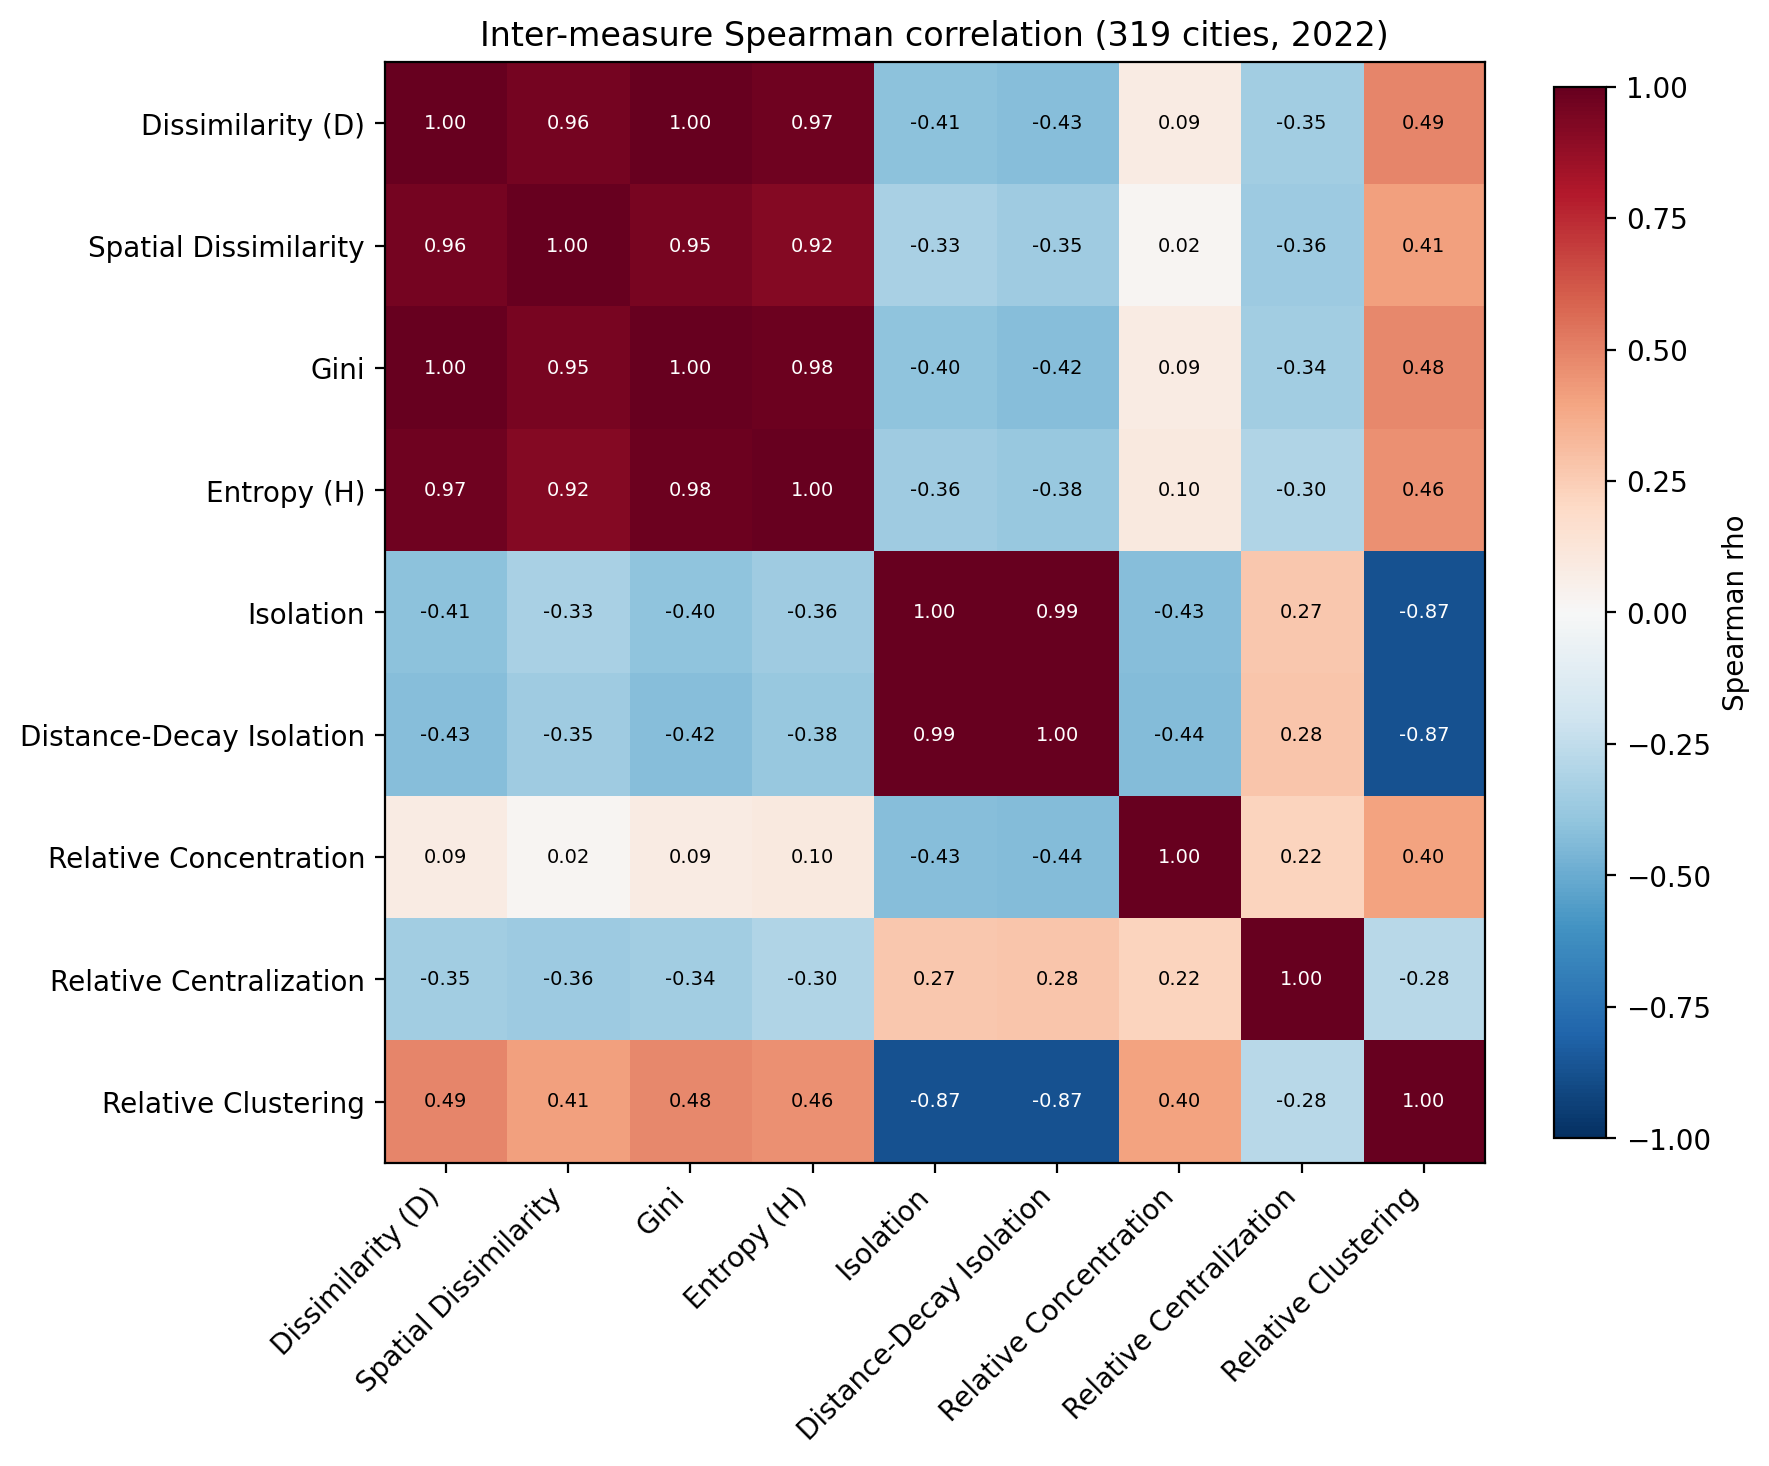
\includegraphics[width=\textwidth]{fig_correlation.png}
\caption{Correlation matrix of segregation measures across cities.}
\label{fig:correlation}
\end{figure}

\begin{figure}[h]
\centering
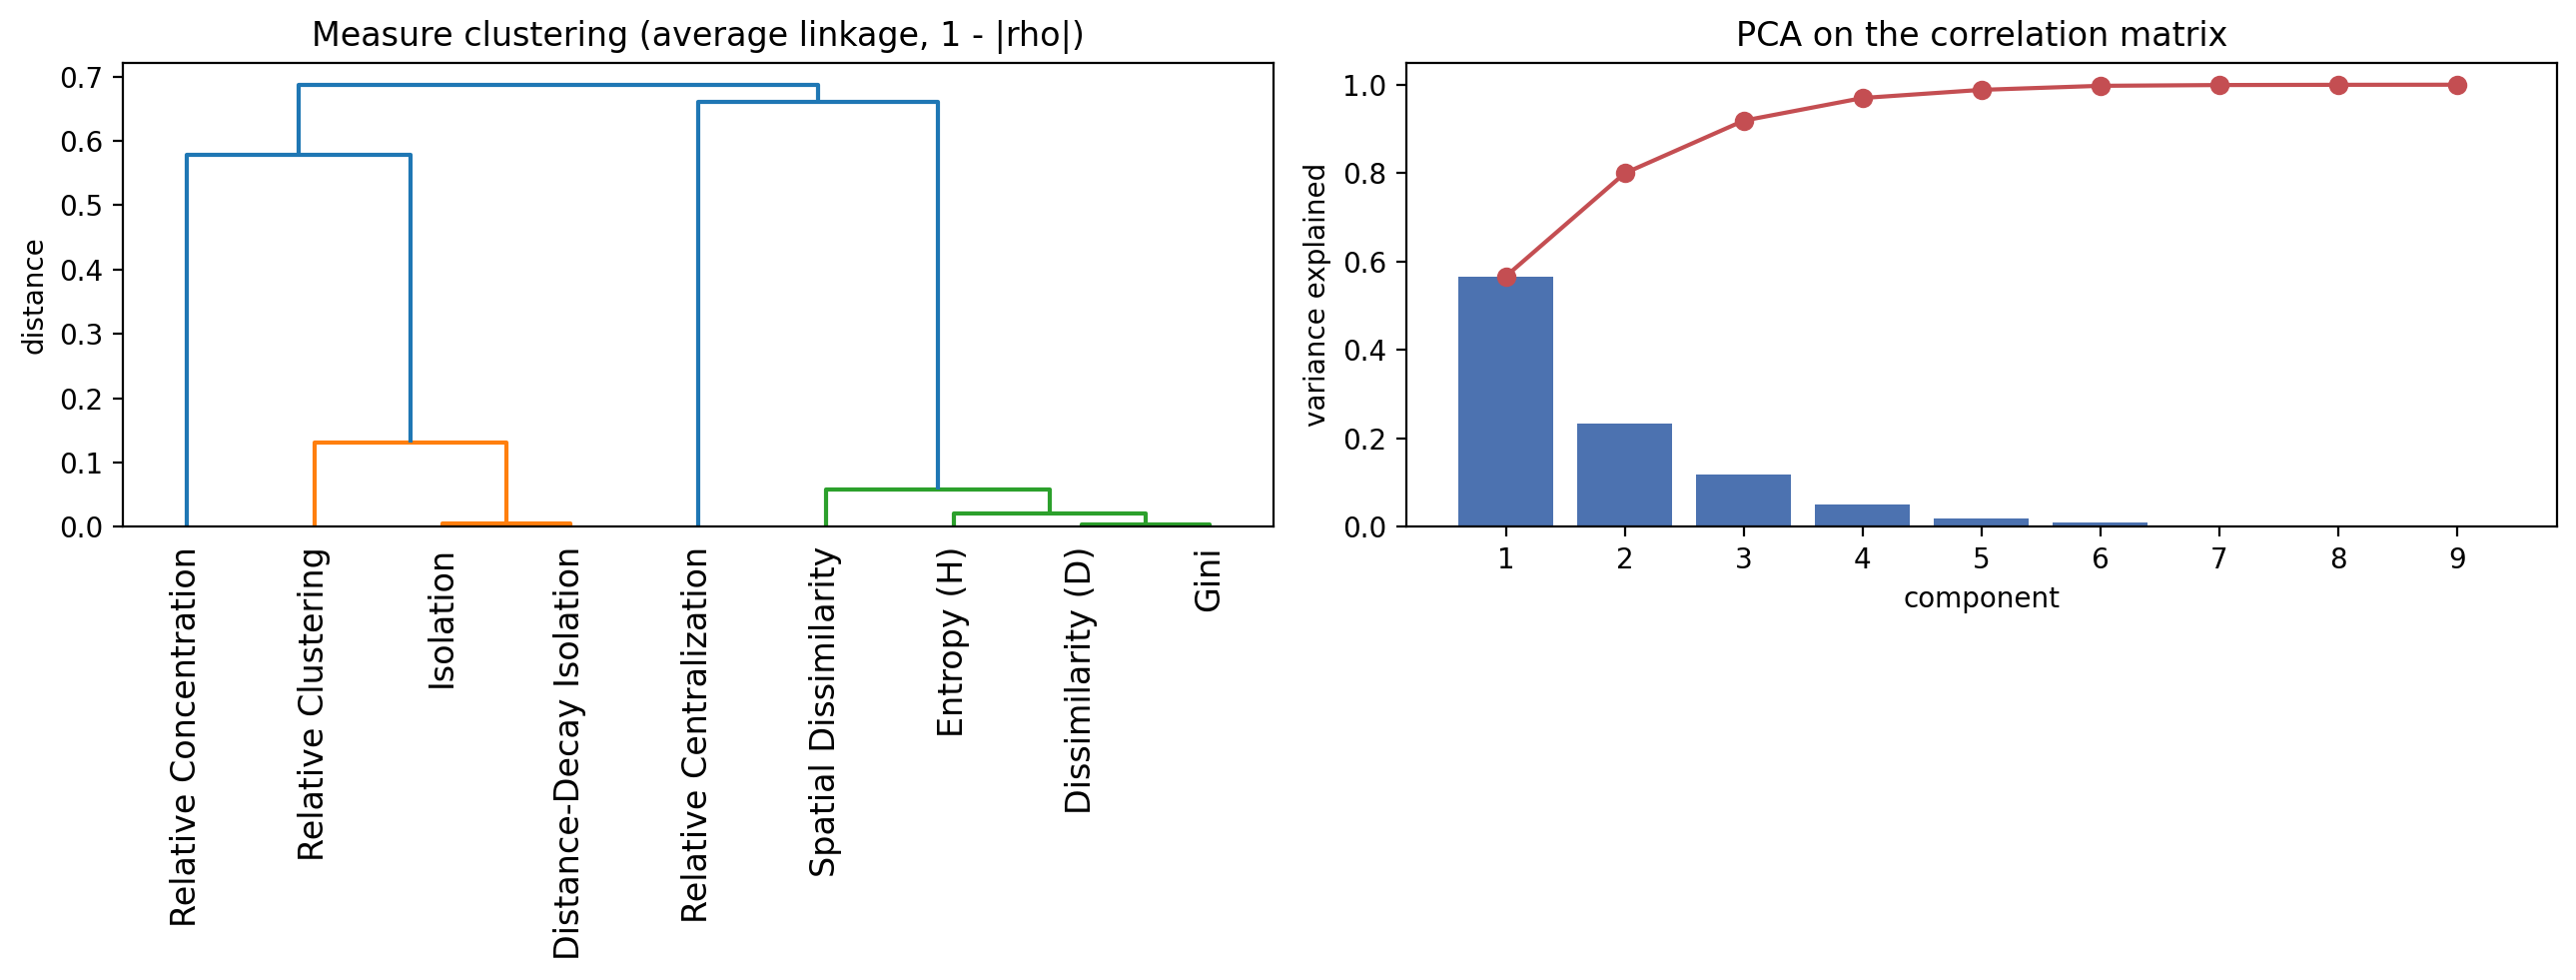
\includegraphics[width=\textwidth]{fig_measure_clustering.png}
\caption{Clustering dimension of segregation measures.}
\label{fig:clustering}
\end{figure}

\begin{table}
\caption{Correlação de Spearman entre os nove índices de segregação (nível cidade, Censo 2022). Colunas: D=Dissimilaridade, SD=Dissimilaridade espacial, G=Gini, H=Entropia, Iso=Isolamento, DDI=Isolamento com decaimento, RCo=Concentração relativa, RCe=Centralização relativa, RCl=Agrupamento relativo.}
\label{tab:corr}
\begin{tabular}{lrrrrrrrrr}
\toprule
 & D & SD & G & H & Iso & DDI & RCo & RCe & RCl \\
Medida &  &  &  &  &  &  &  &  &  \\
\midrule
Dissimilarity (D) & 1.00 & 0.96 & 1.00 & 0.97 & -0.41 & -0.43 & 0.09 & -0.35 & 0.49 \\
Spatial Dissimilarity & 0.96 & 1.00 & 0.95 & 0.92 & -0.33 & -0.35 & 0.02 & -0.36 & 0.41 \\
Gini & 1.00 & 0.95 & 1.00 & 0.98 & -0.40 & -0.42 & 0.09 & -0.34 & 0.48 \\
Entropy (H) & 0.97 & 0.92 & 0.98 & 1.00 & -0.36 & -0.38 & 0.10 & -0.30 & 0.46 \\
Isolation & -0.41 & -0.33 & -0.40 & -0.36 & 1.00 & 0.99 & -0.43 & 0.27 & -0.87 \\
Distance-Decay Isolation & -0.43 & -0.35 & -0.42 & -0.38 & 0.99 & 1.00 & -0.44 & 0.28 & -0.87 \\
Relative Concentration & 0.09 & 0.02 & 0.09 & 0.10 & -0.43 & -0.44 & 1.00 & 0.22 & 0.40 \\
Relative Centralization & -0.35 & -0.36 & -0.34 & -0.30 & 0.27 & 0.28 & 0.22 & 1.00 & -0.28 \\
Relative Clustering & 0.49 & 0.41 & 0.48 & 0.46 & -0.87 & -0.87 & 0.40 & -0.28 & 1.00 \\
\bottomrule
\end{tabular}
\end{table}


\subsection{Which cities are most segregated?}\label{sec:rank}

\begin{figure}[h]
\centering
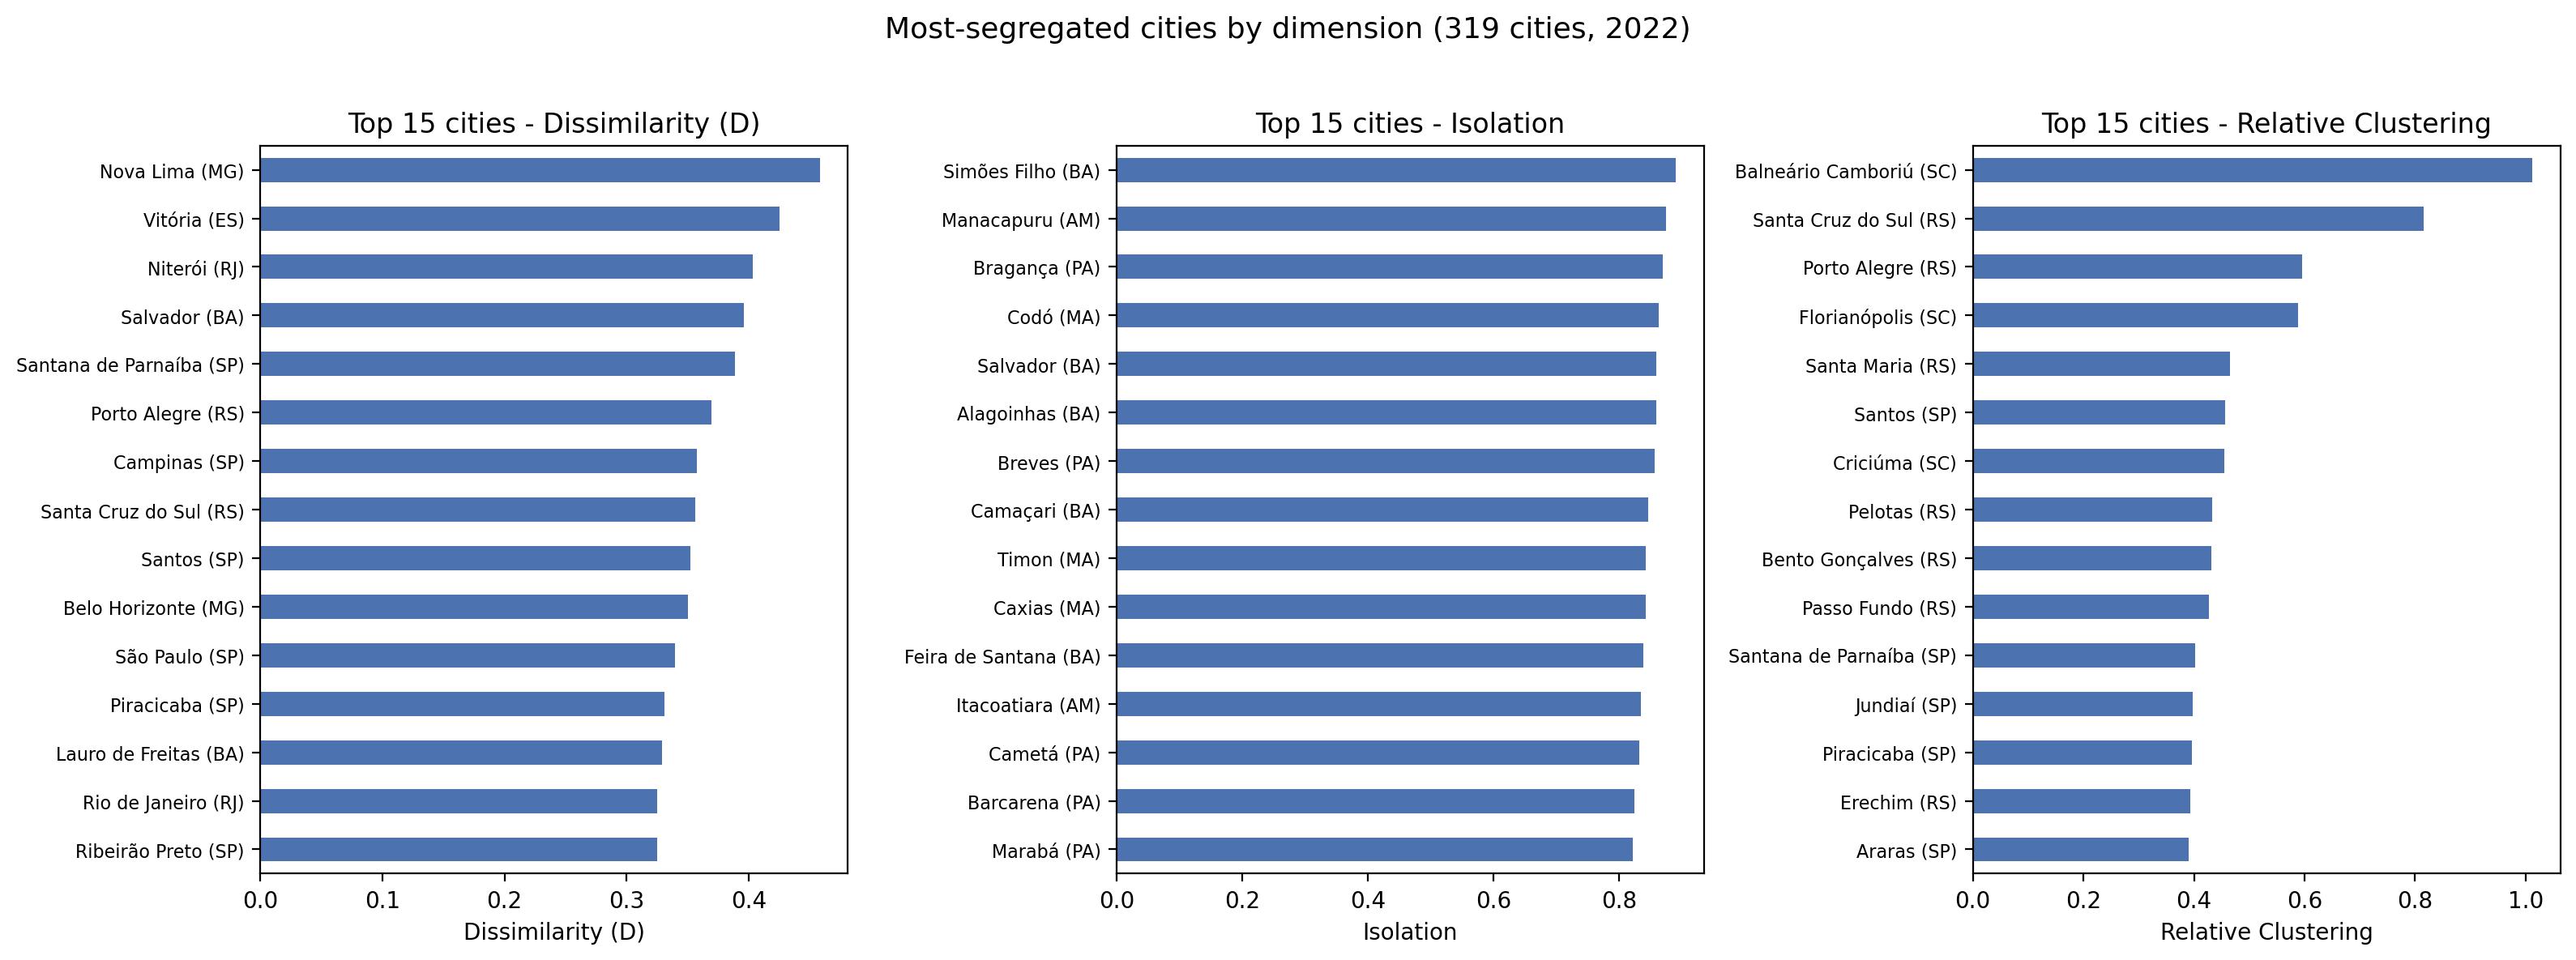
\includegraphics[width=\textwidth]{fig_rankings.png}
\caption{Rankings of cities by segregation indices.}
\label{fig:rankings}
\end{figure}

\begin{table}
\caption{Correlação de postos de Kendall (tau) entre os ordenamentos de cidades pelos nove índices de segregação (nível cidade, Censo 2022). Colunas: D=Dissimilaridade, SD=Dissimilaridade espacial, G=Gini, H=Entropia, Iso=Isolamento, DDI=Isolamento com decaimento, RCo=Concentração relativa, RCe=Centralização relativa, RCl=Agrupamento relativo.}
\label{tab:rankcorr}
\begin{tabular}{lrrrrrrrrr}
\toprule
 & D & SD & G & H & Iso & DDI & RCo & RCe & RCl \\
\midrule
Dissimilarity (D) & 1.00 & 0.83 & 0.96 & 0.89 & -0.26 & -0.28 & 0.06 & -0.25 & 0.35 \\
Spatial Dissimilarity & 0.83 & 1.00 & 0.82 & 0.76 & -0.21 & -0.23 & 0.01 & -0.25 & 0.29 \\
Gini & 0.96 & 0.82 & 1.00 & 0.91 & -0.26 & -0.27 & 0.06 & -0.24 & 0.34 \\
Entropy (H) & 0.89 & 0.76 & 0.91 & 1.00 & -0.23 & -0.25 & 0.06 & -0.22 & 0.32 \\
Isolation & -0.26 & -0.21 & -0.26 & -0.23 & 1.00 & 0.94 & -0.30 & 0.18 & -0.67 \\
Distance-Decay Isolation & -0.28 & -0.23 & -0.27 & -0.25 & 0.94 & 1.00 & -0.30 & 0.18 & -0.68 \\
Relative Concentration & 0.06 & 0.01 & 0.06 & 0.06 & -0.30 & -0.30 & 1.00 & 0.15 & 0.27 \\
Relative Centralization & -0.25 & -0.25 & -0.24 & -0.22 & 0.18 & 0.18 & 0.15 & 1.00 & -0.19 \\
Relative Clustering & 0.35 & 0.29 & 0.34 & 0.32 & -0.67 & -0.68 & 0.27 & -0.19 & 1.00 \\
\bottomrule
\end{tabular}
\end{table}


\subsection{Regional patterns}\label{sec:region}

\begin{figure}[h]
\centering

\includegraphics[width=\textwidth]{fig_regional.png}
\caption{Regional variation in segregation measures.}
\label{fig:regional}
\end{figure}

\begin{table}
\caption{Mediana de cada índice de segregação por macrorregião (nível cidade, Censo 2022). Colunas: D=Dissimilaridade, SD=Dissimilaridade espacial, G=Gini, H=Entropia, Iso=Isolamento, DDI=Isolamento com decaimento, RCo=Concentração relativa, RCe=Centralização relativa, RCl=Agrupamento relativo.}
\label{tab:regional}
\begin{tabular}{lrrrrrrrrr}
\toprule
 & D & SD & G & H & Iso & DDI & RCo & RCe & RCl \\
Região &  &  &  &  &  &  &  &  &  \\
\midrule
Norte & 0.176 & 0.108 & 0.256 & 0.041 & 0.790 & 0.832 & -0.649 & -0.061 & -0.058 \\
Nordeste & 0.171 & 0.106 & 0.246 & 0.034 & 0.741 & 0.764 & -0.303 & -0.045 & -0.065 \\
Centro-Oeste & 0.177 & 0.098 & 0.252 & 0.037 & 0.644 & 0.682 & -0.144 & -0.068 & 0.015 \\
Sudeste & 0.219 & 0.128 & 0.306 & 0.055 & 0.537 & 0.529 & -0.063 & -0.082 & 0.093 \\
Sul & 0.217 & 0.136 & 0.299 & 0.051 & 0.329 & 0.323 & 0.096 & -0.069 & 0.206 \\
\bottomrule
\end{tabular}
\end{table}


\subsection{Minority share and segregation}\label{sec:share}

\begin{figure}[h]
\centering

\includegraphics[width=\textwidth]{fig_minorityshare.png}
\caption{Relationship between minority share and segregation.}
\label{fig:minorityshare}
\end{figure}

\subsection{The spatial texture of segregation}\label{sec:maps}

\begin{figure}[h]
\centering
\begin{subfigure}[b]{0.48\textwidth}
\centering
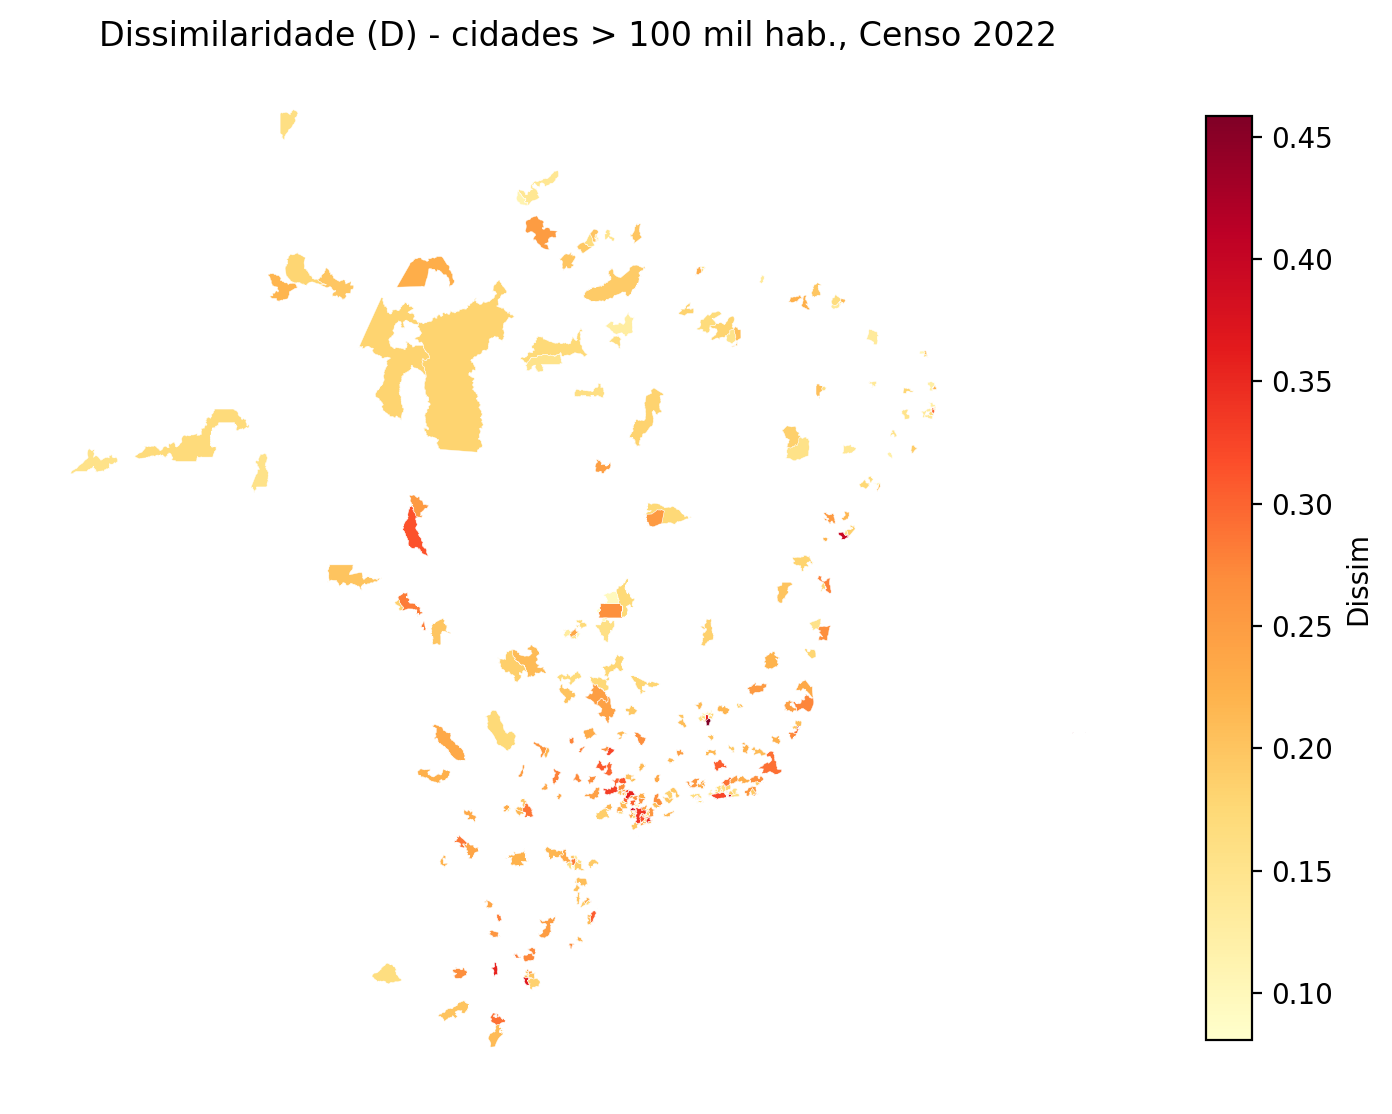
\includegraphics[width=\textwidth]{fig_map_national_dissim.png}
\caption{Dissimilarity index}
\label{fig:map-dissim}
\end{subfigure}
\hfill
\begin{subfigure}[b]{0.48\textwidth}
\centering
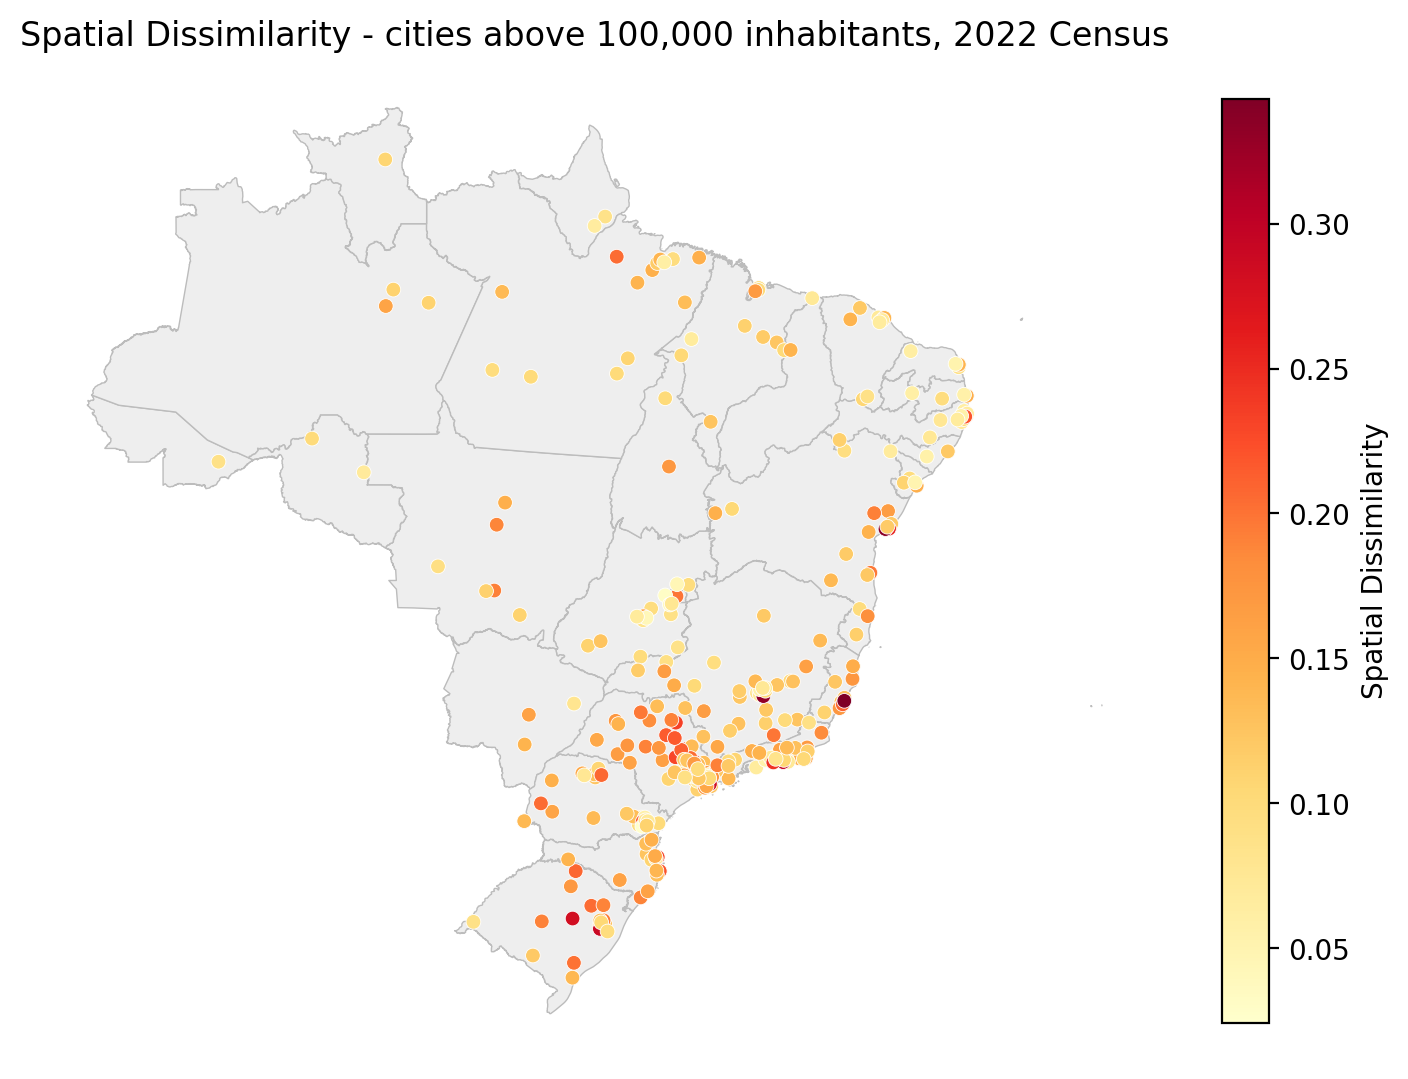
\includegraphics[width=\textwidth]{fig_map_national_spatial.png}
\caption{Spatial clustering}
\label{fig:map-spatial}
\end{subfigure}
\caption{National-scale maps of racial residential segregation.}
\label{fig:maps-national}
\end{figure}

\begin{figure}[h]
\centering
\begin{subfigure}[b]{0.32\textwidth}
\centering
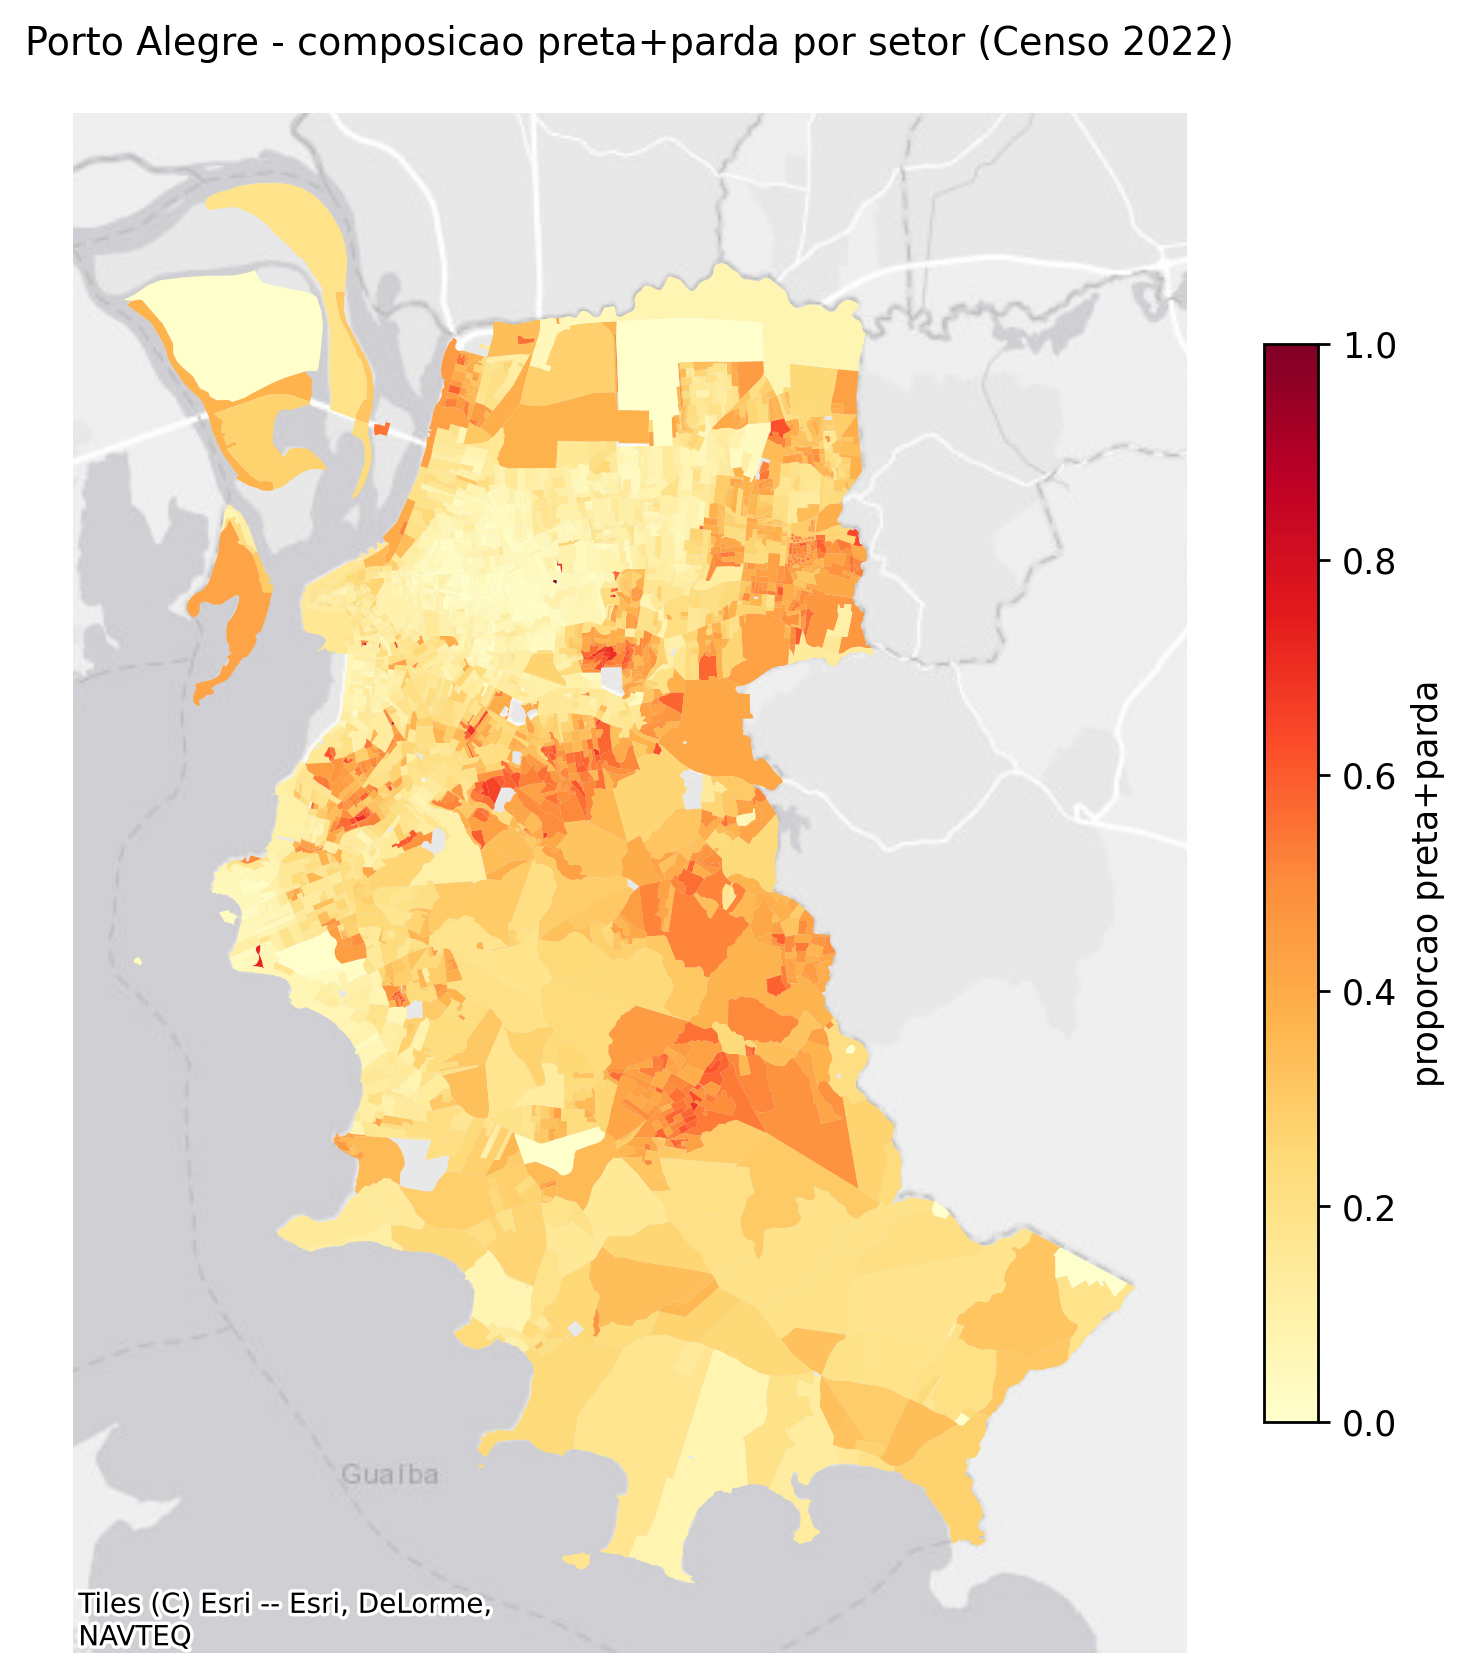
\includegraphics[width=\textwidth]{seg_profile_4314902.png}
\caption{Porto Alegre}
\label{fig:city-pa}
\end{subfigure}
\hfill
\begin{subfigure}[b]{0.32\textwidth}
\centering
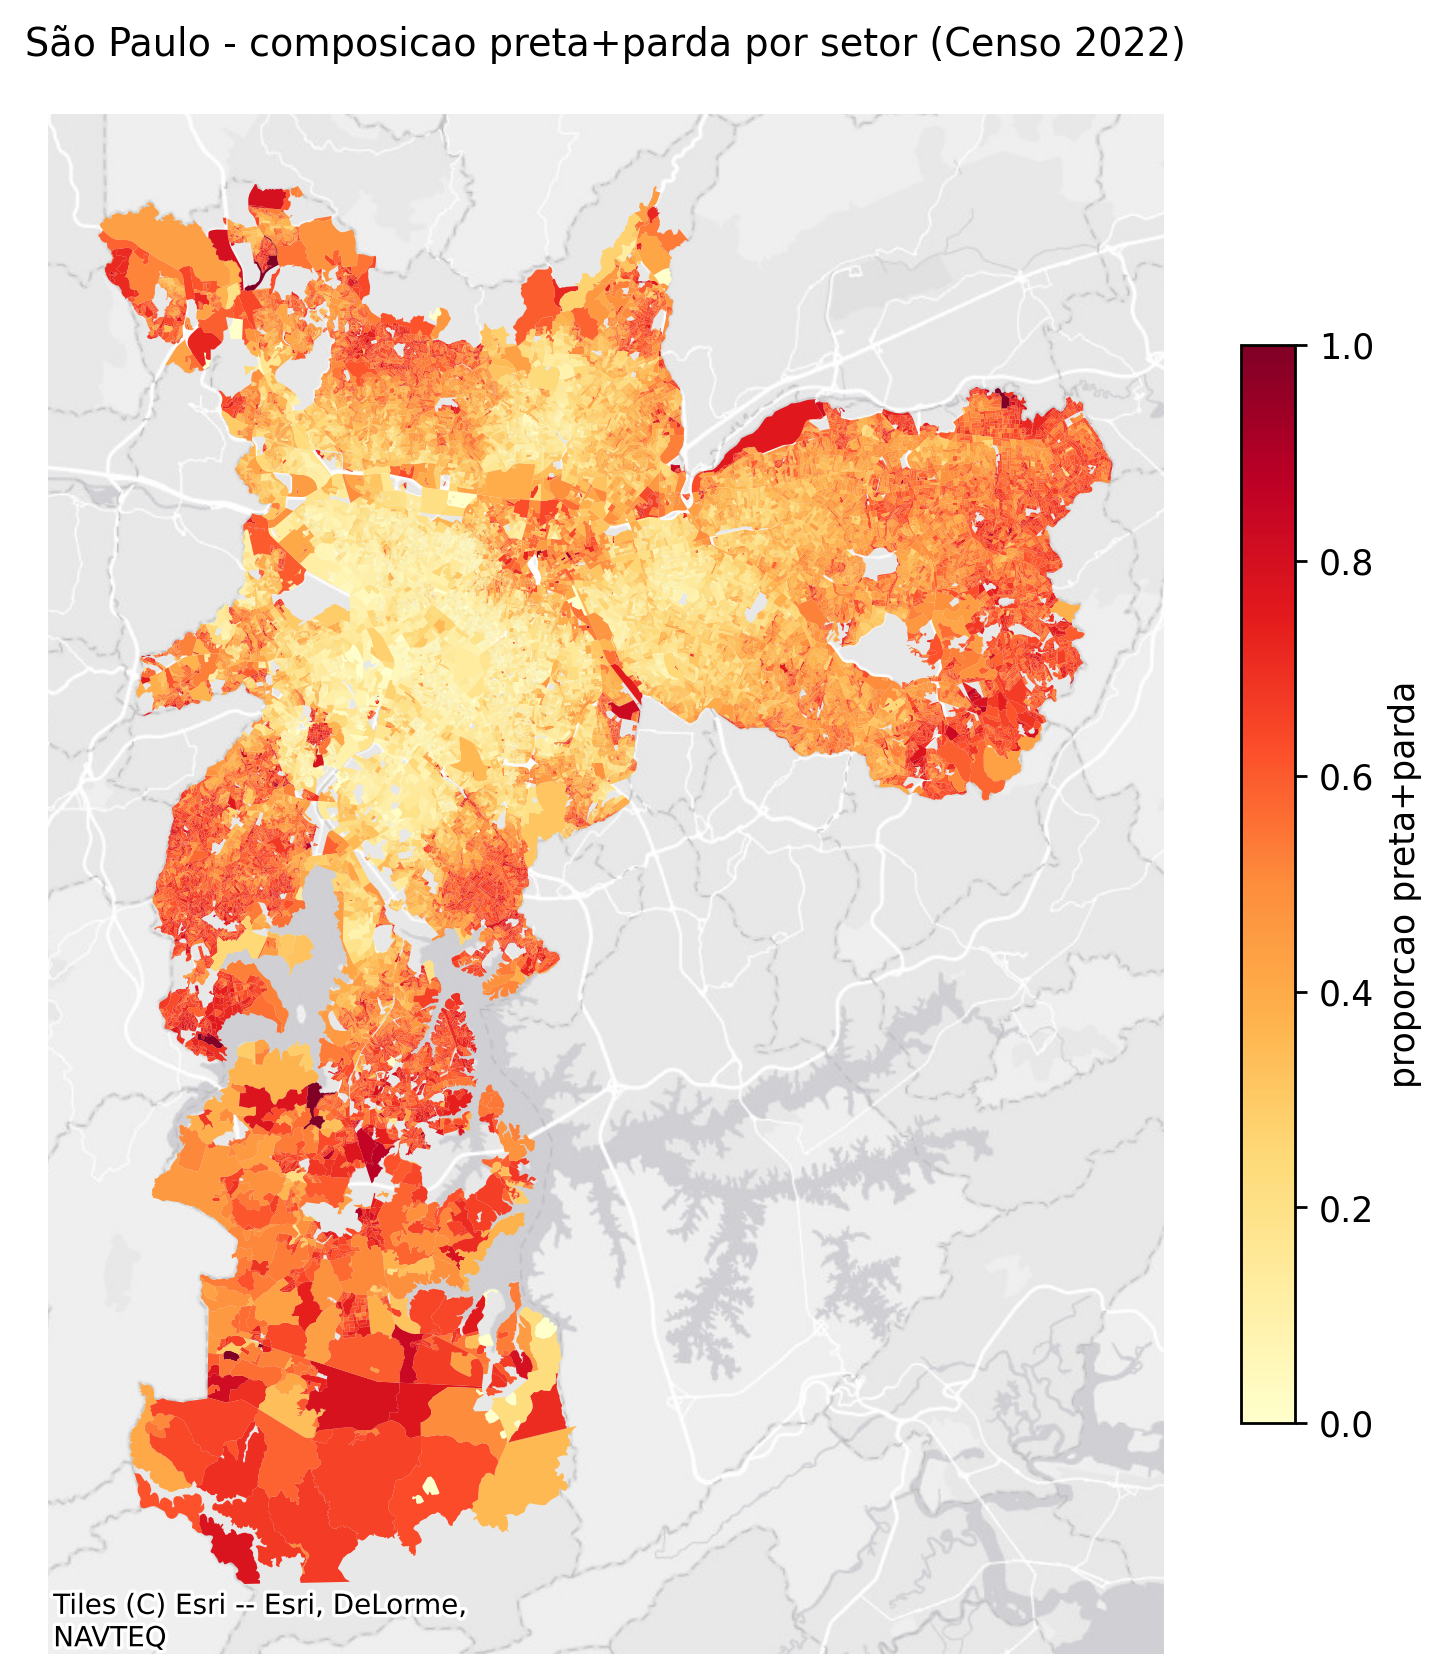
\includegraphics[width=\textwidth]{seg_profile_3550308.png}
\caption{São Paulo}
\label{fig:city-sp}
\end{subfigure}
\hfill
\begin{subfigure}[b]{0.32\textwidth}
\centering
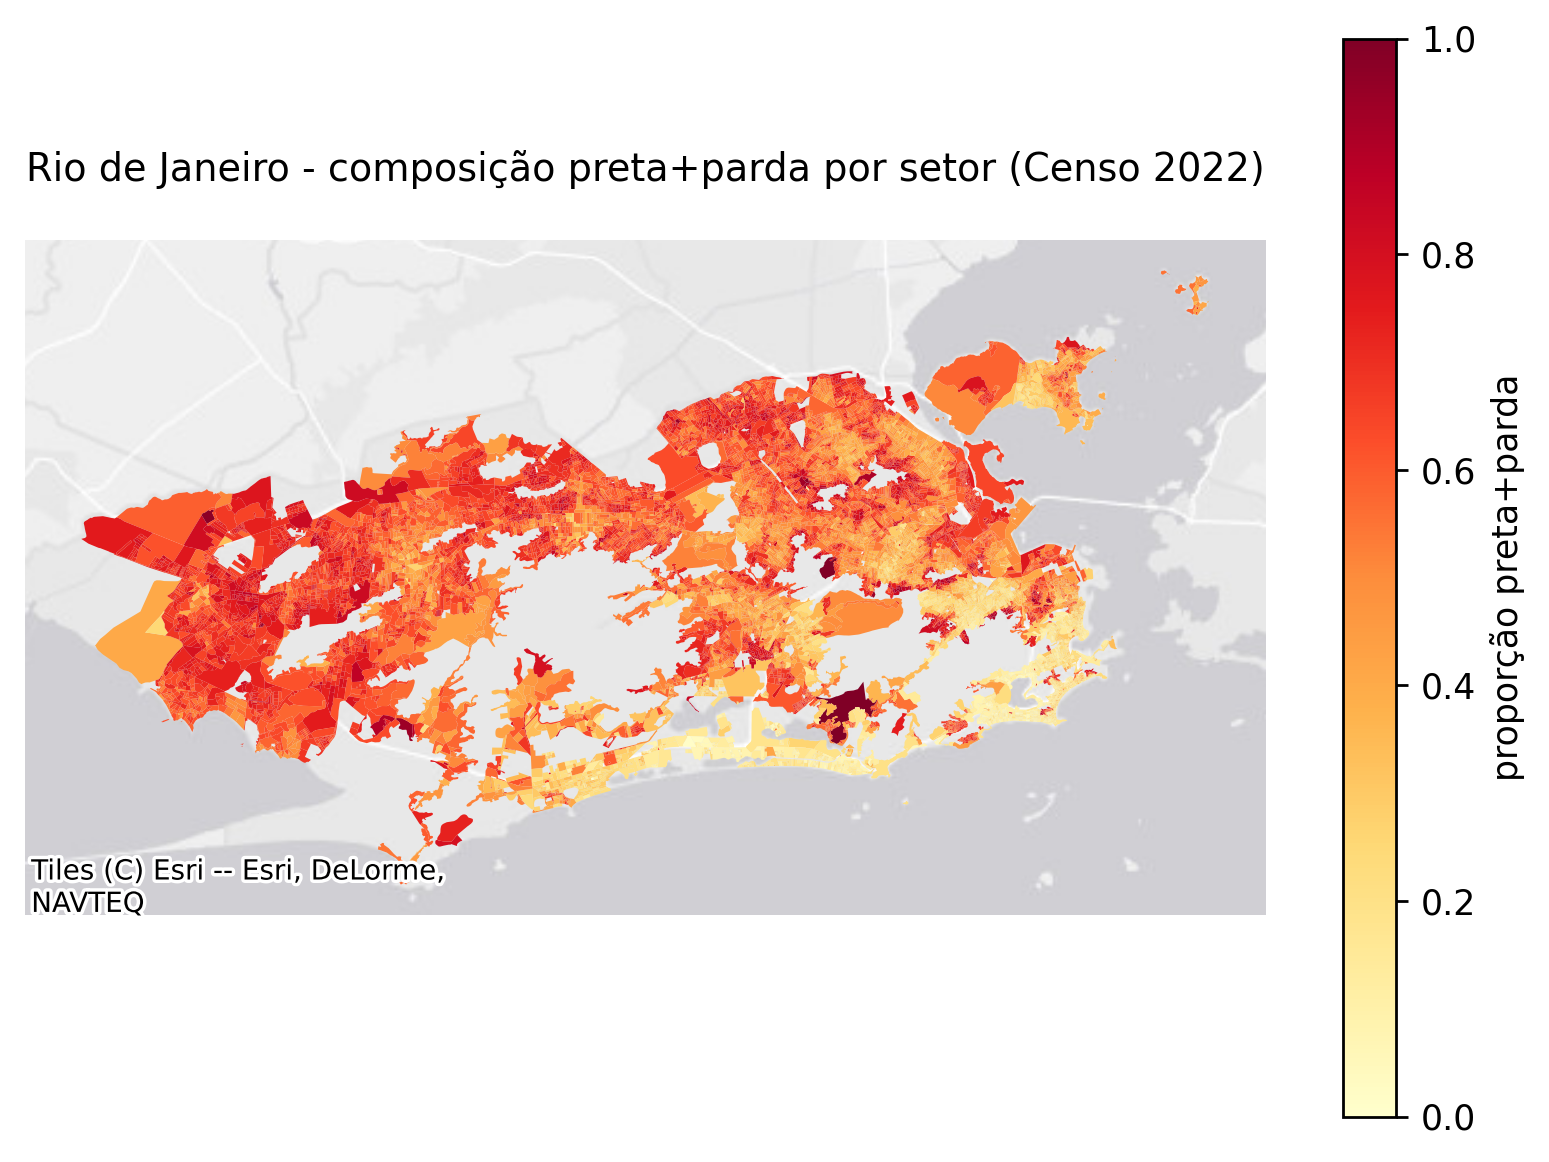
\includegraphics[width=\textwidth]{seg_profile_3304557.png}
\caption{Rio de Janeiro}
\label{fig:city-rj}
\end{subfigure}

\begin{subfigure}[b]{0.32\textwidth}
\centering
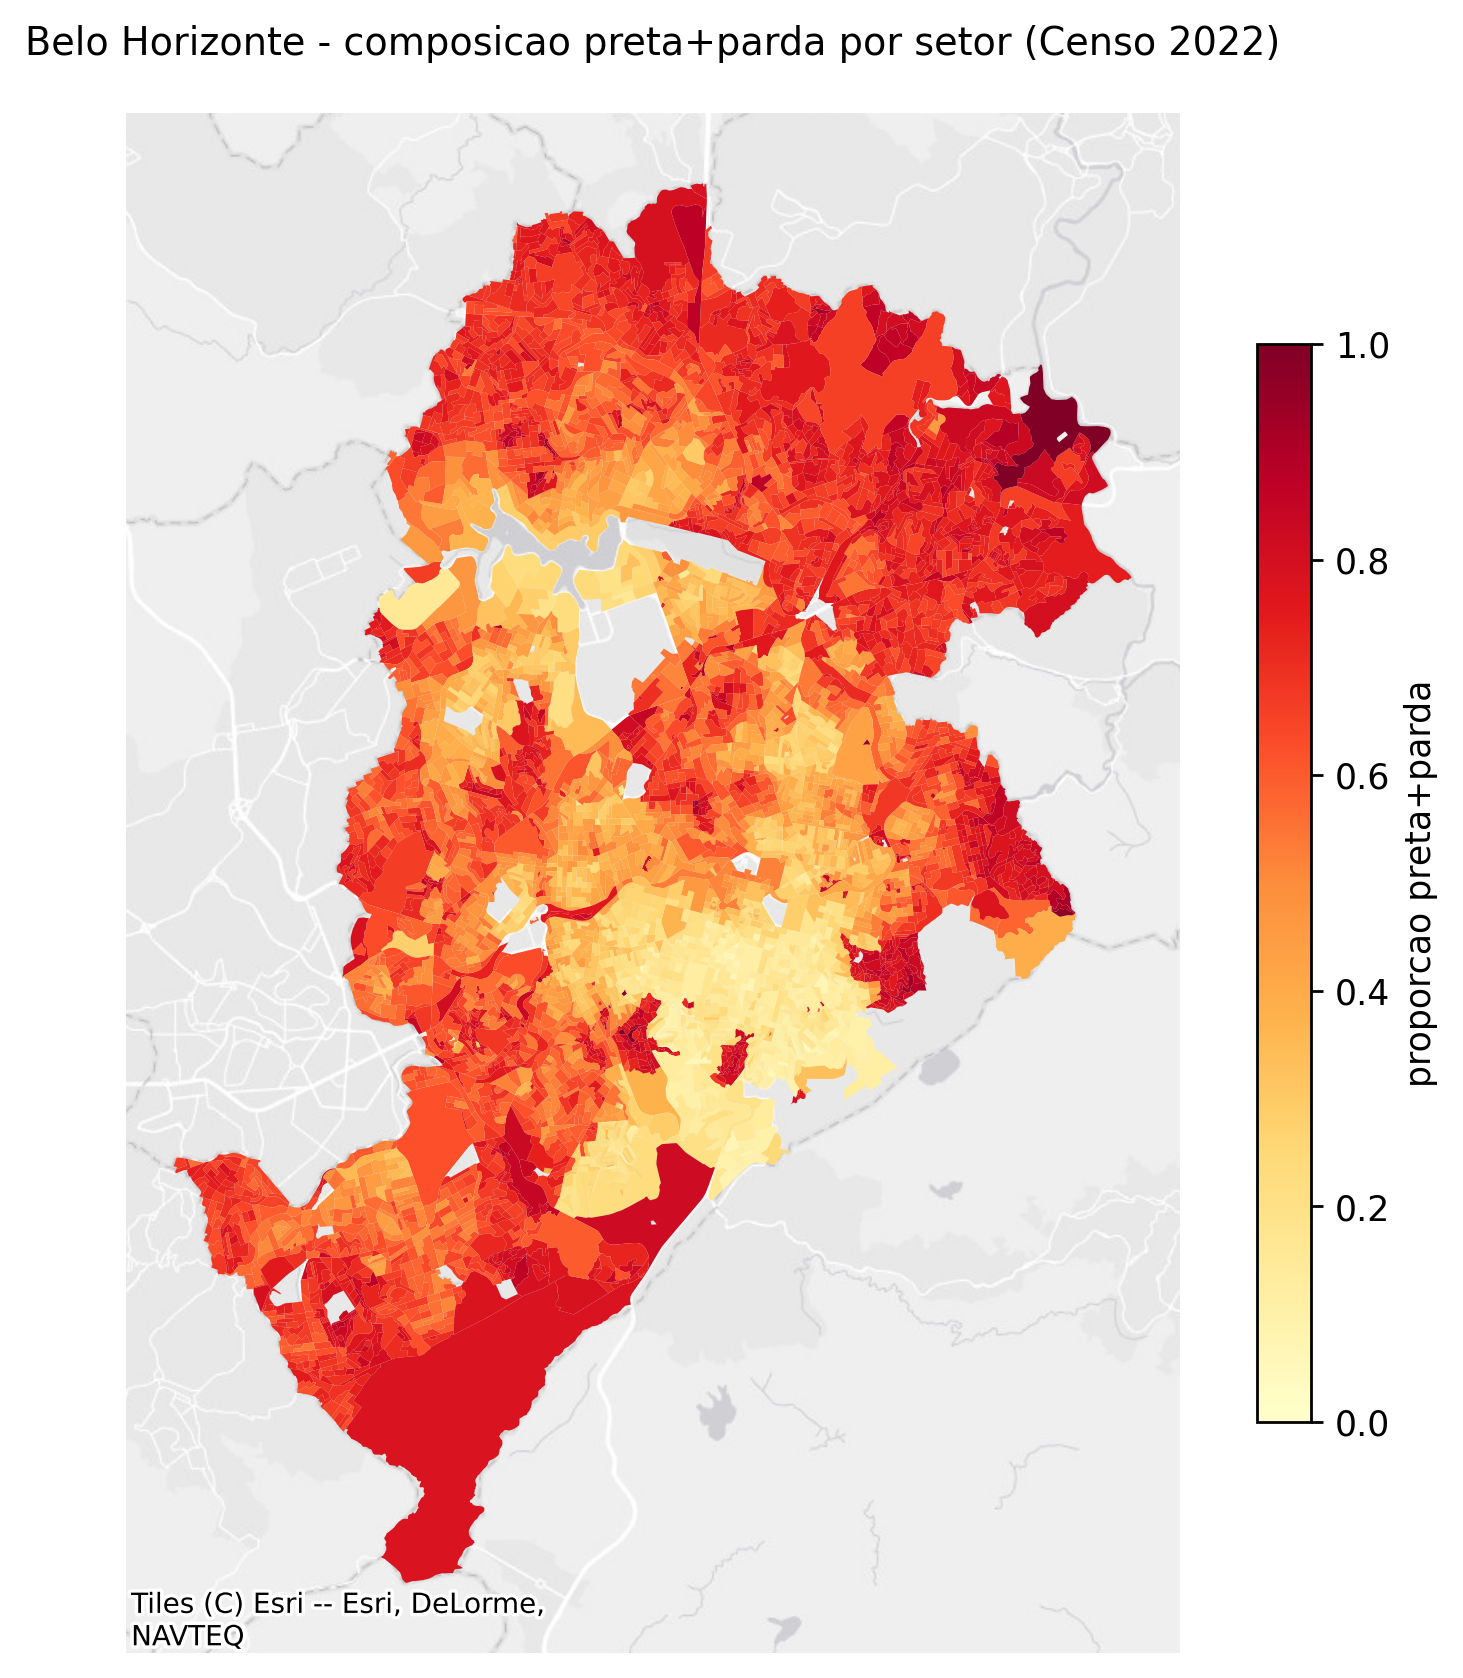
\includegraphics[width=\textwidth]{seg_profile_3106200.png}
\caption{Belo Horizonte}
\label{fig:city-bh}
\end{subfigure}
\hfill
\begin{subfigure}[b]{0.32\textwidth}
\centering
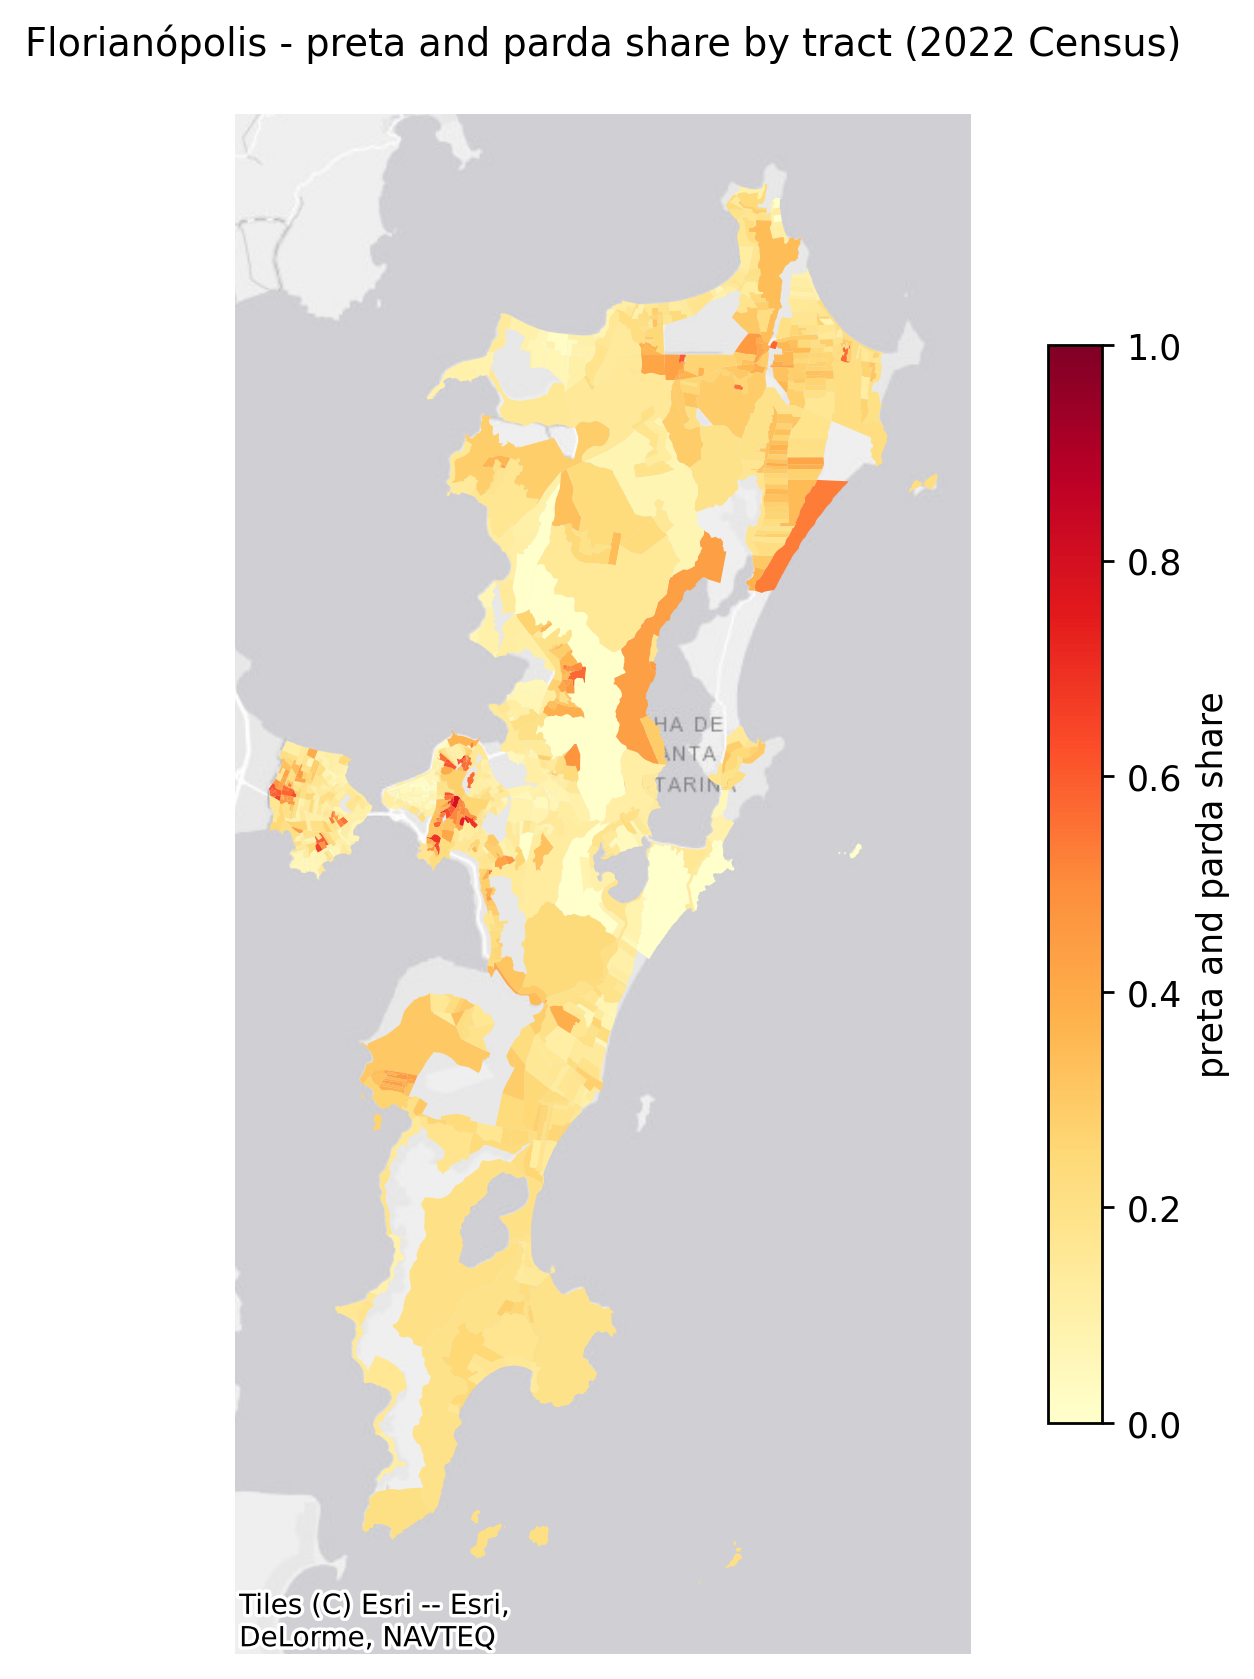
\includegraphics[width=\textwidth]{seg_profile_4205407.png}
\caption{Florianópolis}
\label{fig:city-fl}
\end{subfigure}
\hfill
\begin{subfigure}[b]{0.32\textwidth}
\centering
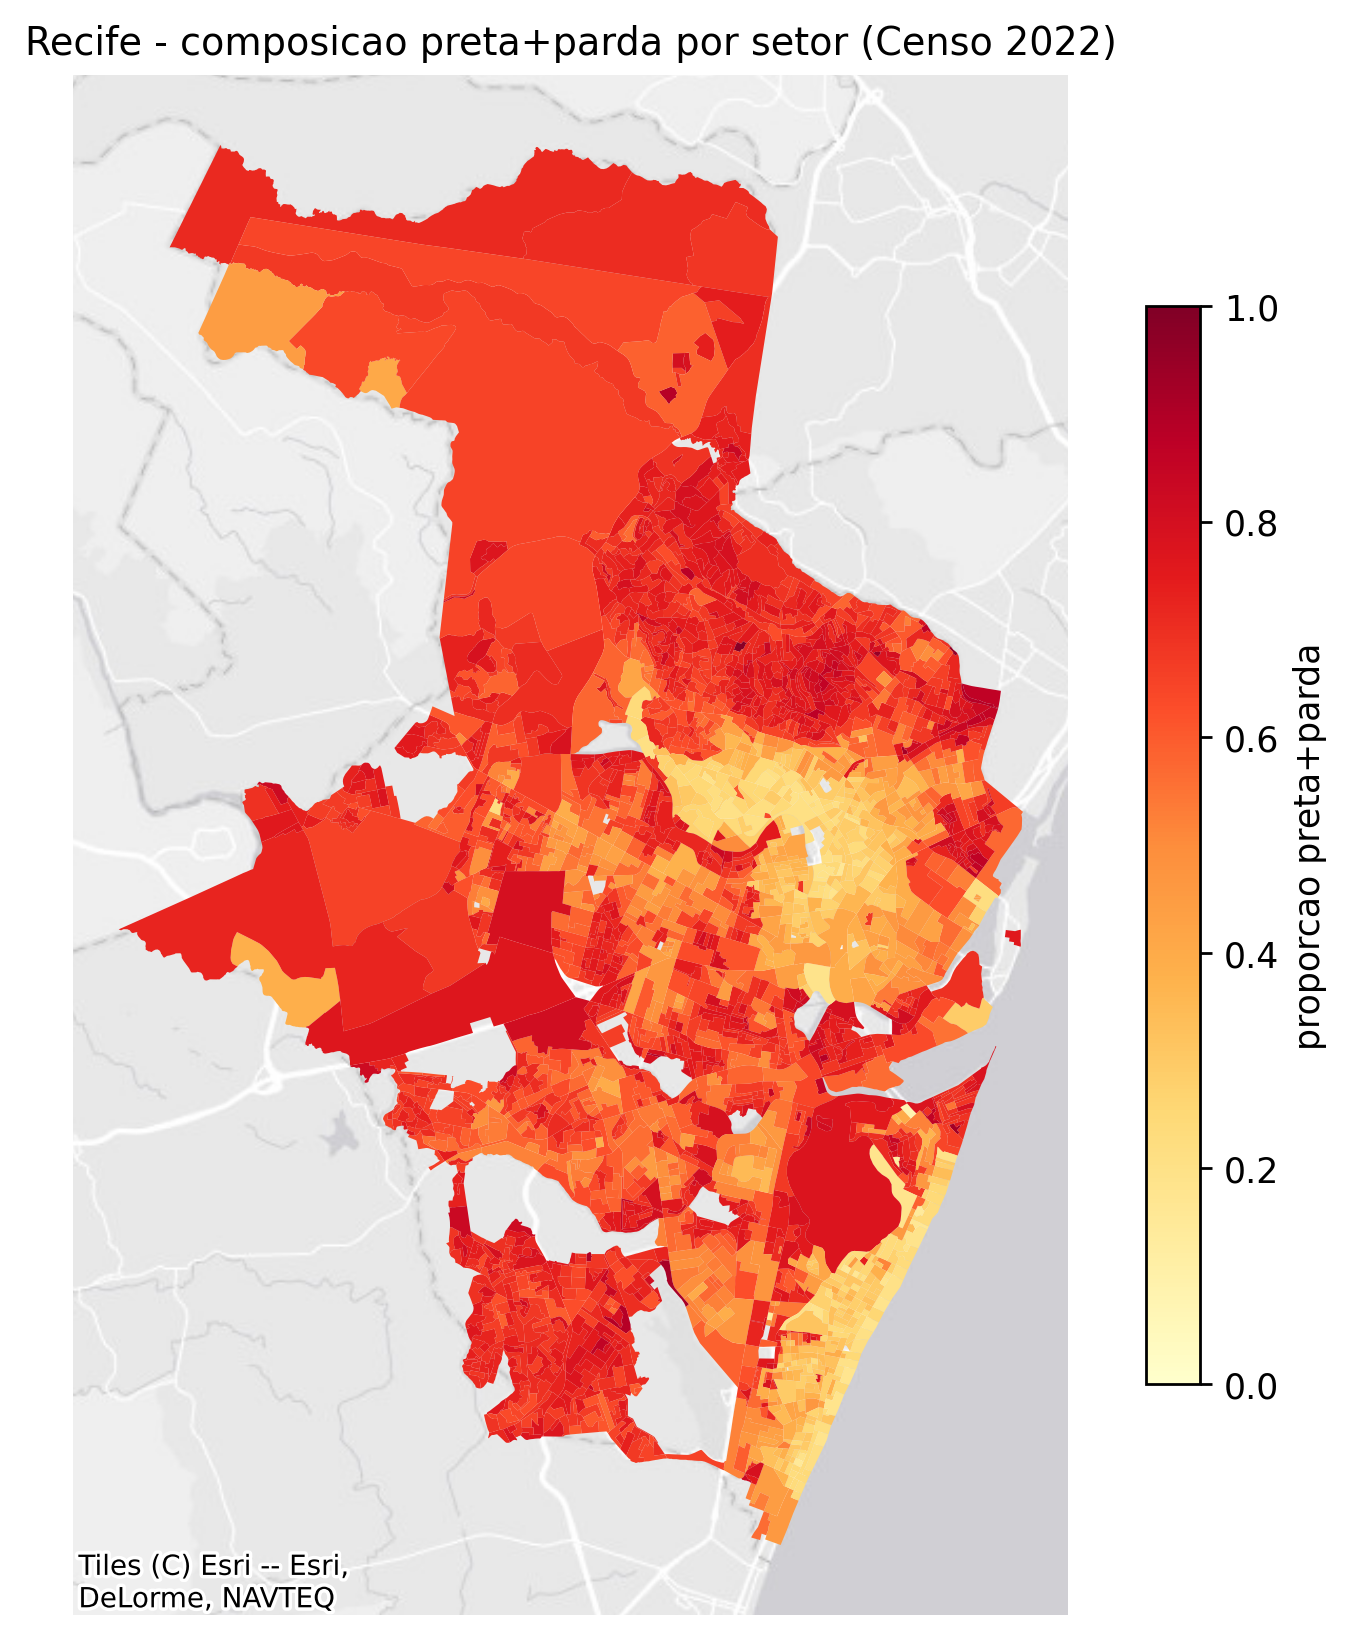
\includegraphics[width=\textwidth]{seg_profile_2611606.png}
\caption{Recife}
\label{fig:city-rc}
\end{subfigure}

\caption{Segregation profiles for six major Brazilian cities.}
\label{fig:maps-cities}
\end{figure}

\section{Discussion}\label{sec:discussion}
% TODO(task22)

\section{Reproducibility}\label{sec:repro}
% TODO(task22)

\section{Conclusion}\label{sec:conclusion}
% TODO(task22)

\bibliographystyle{plainnat}
\bibliography{references}

\end{document}
